\documentclass[ddcfooter]{tudbeamer}
\usepackage{german}
\usepackage{graphicx}
\usepackage{caption}
\usepackage{listings}
\usepackage{setspace}
\usepackage{array}

\usetheme{Antibes}


\usepackage{fontspec}
\usepackage{xltxtra}
\setmainfont{Univers}
\setmonofont{Courier}
\setromanfont{Univers}
\setsansfont{Ubuntu}

\begin{document}

\einrichtung{Fakultät Informatik\hspace{6cm} Institut für Systemarchitektur}
\title[Speicherverwaltung in Linux]{Vortrag im Proseminar Betriebssysteme:\vfill Speicherverwaltung in Linux}
\author{Rebecca Kratsch}

\date{10.05.2013}

\maketitle



\begin{frame}
    \frametitle{Inhalt}
    \begin{itemize}
	\item Grundlegende Konzepte
	\item Verwaltung des physischen Speichers
	\begin{itemize}
	    \item Speicherbelegung am Beispiel des Buddy-Algorithmus
	\end{itemize}
	    \item Repräsentation des virtuellen Speichers
	\begin{itemize}
	    \item Paging
	    \item Seitenersetzungsalgorithmus
	\end{itemize}
    \end{itemize}
\end{frame}



\section{Grundlegendes}
\begin{frame} 
    \frametitle{Grundlegendes}
    
    Bild zu Thema fehlt noch\\
    
    \begin{itemize}
    	\item Stack: 
		\begin{itemize}
			\item Umgebungsvariablen, Kommandozeile
			\item veränderbar
		\end{itemize}
	\item Datensegment: (Bild : BSS und Daten) 
		\begin{itemize}
			\item initialisierte Daten    
			\item uninitialisierte Daten ( Verweis auf Zeropage)
		\end{itemize}
	\item Textsegment: 
		\begin{itemize}
			\item Maschinenbefehle
			\item nur lesender Zugriff
			\item keine Größenänderung mögl. 
		\end{itemize}
    \end{itemize}
   
%\renewcommand{\arraystretch}{1.2}
%{\tiny
%\begin{tabular}{ | c | c | m{5cm} |}
    %	\cline{1-1} \cline{3-3} 
	%Stack &  &   \\ \cline{1-1} \cline{3-3}
	    %  &  &   \\ \cline{1-1} \cline{3-3}               &  &   \\ \cline{1-1} \cline{3-3}
	  %    &  &   \\ \cline{1-1} \cline{3-3}
	      %&  &   \\ \cline{1-1} \cline{3-3}
            %  &  &   \\ \cline{1-1} \cline{3-3}
	    %  &  &   \\ \cline{1-1} \cline{3-3}
	  %    &  &   \\ \cline{1-1} \cline{3-3}
	      %&  &   \\ \cline{1-1} \cline{3-3}
%	      &  &   \\ \cline{1-1} \cline{3-3}
%	      &  &   \\ \cline{1-1} \cline{3-3}
%	      &  &   \\ \cline{1-1} \cline{3-3}
%	      &  &   \\ \cline{1-1} \cline{3-3}
%	      &  &   \\ \cline{1-1} \cline{3-3}
%	      &  &   \\ \cline{1-1} \cline{3-3}
%	BSS   &  &   \\ \cline{1-1} \cline{3-3} 
%	Daten &  &   \\ \cline{1-1} \cline{3-3}    
%	Daten &  &   \\ \cline{1-1} \cline{3-3} 
%	Text  &  &   \\ \cline{1-1} \cline{3-3}  
%	
%    \end{tabular}
%}
%\renewcommand{\arraystrech}{1}

\end{frame}

\begin{frame} 
    \frametitle{Grundlegendes}
    \framesubtitle{Shared Text Segment}
    
    Grafik....
    
    
    
    
\end{frame}

\begin{frame} 
    \frametitle{Grundlegendes}
    \framesubtitle{Memory-Mapped-Dateien}
    
    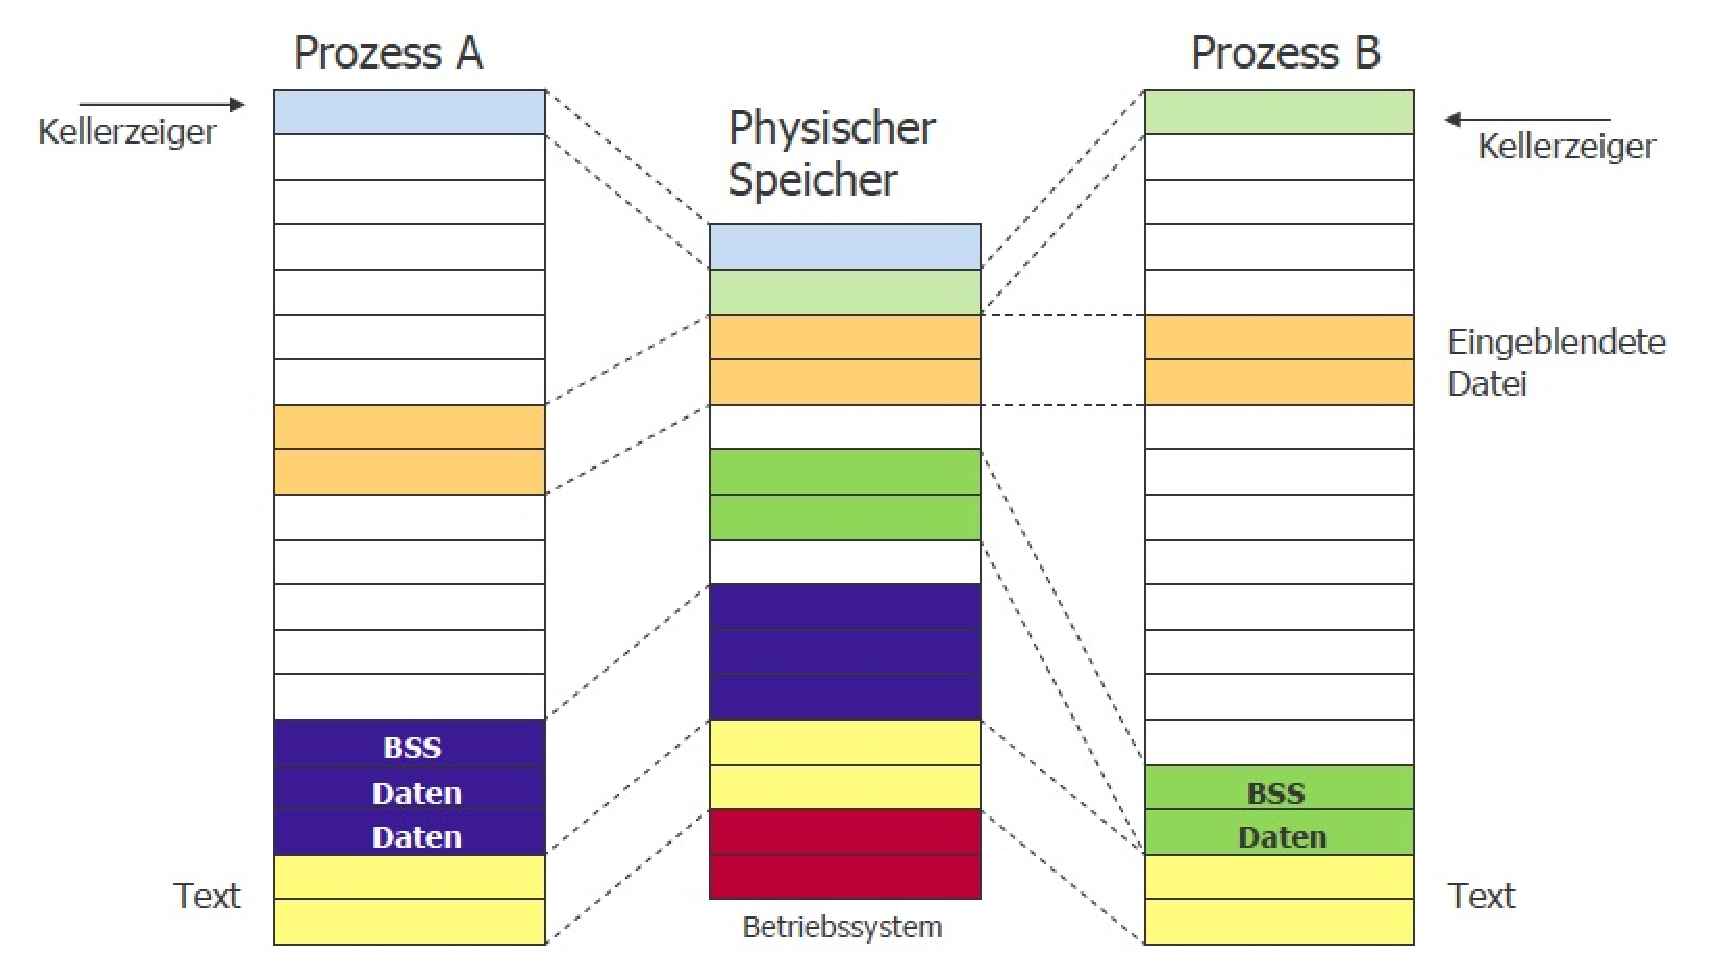
\includegraphics[width=9cm]{segmente.eps}
    
    
    
    
\end{frame}

\section{Implementierung der Speicherverwaltung}
%\begin{frame}
%    \frametitle{was ihr wollt}
%   
%   \begin{itemize}
%         		\item 3 Speicherzonen: ( Grafik noch einfügen)
%
%		\begin{itemize}
%			\item 1 Zone_DMA
%			\item 2 Zone_Normal
%			\item 3 Zone_Highmen
%		\end{itemize}
%   	\end{itemize} 
%\end{frame}

\begin{frame}
    \frametitle{noch unklar}
   
   \begin{itemize}
         		\item Seitendekriptor
		\item Zonendeskriptor
		\item Knotendeskriptor\\
			
			----eventuell mit Grafik--
			
	
   	\end{itemize} 

   
       
\end{frame}



\section{Systemaufrufe}
\begin{frame}
    \frametitle{Systemaufrufe zur Speicherverwaltung}
   
    \begin{center}
   	 \begin{tabular}{ | l |m{5cm} |}
   	 \hline
   	 Systemaufruf & Beschreibung \\ \hline
    	s= brk(addr) & Datensegmentgröße ändern \\ \hline
    	a = mmap(addr, len, prot, flags, fd, offset)&  Datei einblenden \\ \hline
    	s = munmap(addr, len)  & Dateieinblendung beenden\\ \hline
    	\end{tabular}
    \end{center} 
       
\end{frame}





\section{virtueller Speicher}
\begin{frame}
    \frametitle{Repräsentation des virtuellen Adressraumes}
    \framesubtitle{Grundlegendes}
    \begin{itemize}
         \item   Unterteilung in homogene, zusammenhängende, an Seitengrenzen ausgerichtete 			Regionen
         \item fixe Seitengröße, erweiterbar durch PAE
         \item Beschreibung jedes Kernbereichs mit \texttt{vm\_area\_struct}-Eintrag 
         \begin{itemize}
         		\item sortiert und zusammengefasst nach virtueller Adresse\\
		\item enthält Eigenschaften (Schutzrechte...)
			--> Realisiserung Copy- on-Write
		\item Angaben über Hintergrundspeicher
    		\item Zugriff auf alle Elemenete eines Adressraumes via Speicher-Deskriptor
		\begin{itemize}
			\item verkette Liste
			\item binärer Rot-Schwarz-Baum
		\end{itemize}
   	\end{itemize} 
     \end{itemize}
    
\end{frame}

%\section{virtueller Speicher}
\begin{frame}
    \frametitle{Repräsentation des virtuellen Adressraumes}
    \framesubtitle {Paging in Linux}
    \begin{itemize}
         \item  Grundeinheit: Seite
         \item Grundidee / Definition Paging: \\
        \begin{quote}
         \textquotedblleft
         Paging ist ein Speicherverwaltungsverfahren, das auf der Strukturierung  des virtuellen Speichers 	in Seiten und der Strukturierung des realen Speichers in Seitenrahmen beruht.
    	\textquotedblright \footnote {EHSES, E. u.a. : Betriebssysteme- Ein Lehrbuch mit Übungen zur   	Systemrogrammierung in UNIX/Linux. 3. Aufl. München: Pearson Studium Verlag, 2005, S.294  }
	\end{quote}
 	
	
    
    
     \end{itemize}
    
\end{frame}


\begin{frame}
    \frametitle{Repräsentation des virtuellen Adressraumes}
    \framesubtitle {Paging in Linux}
    \begin{itemize}
         \item Nutzung 4-stufiger Seitentabellen in Linux\\
         --------Grafik überarbeiten ----------
	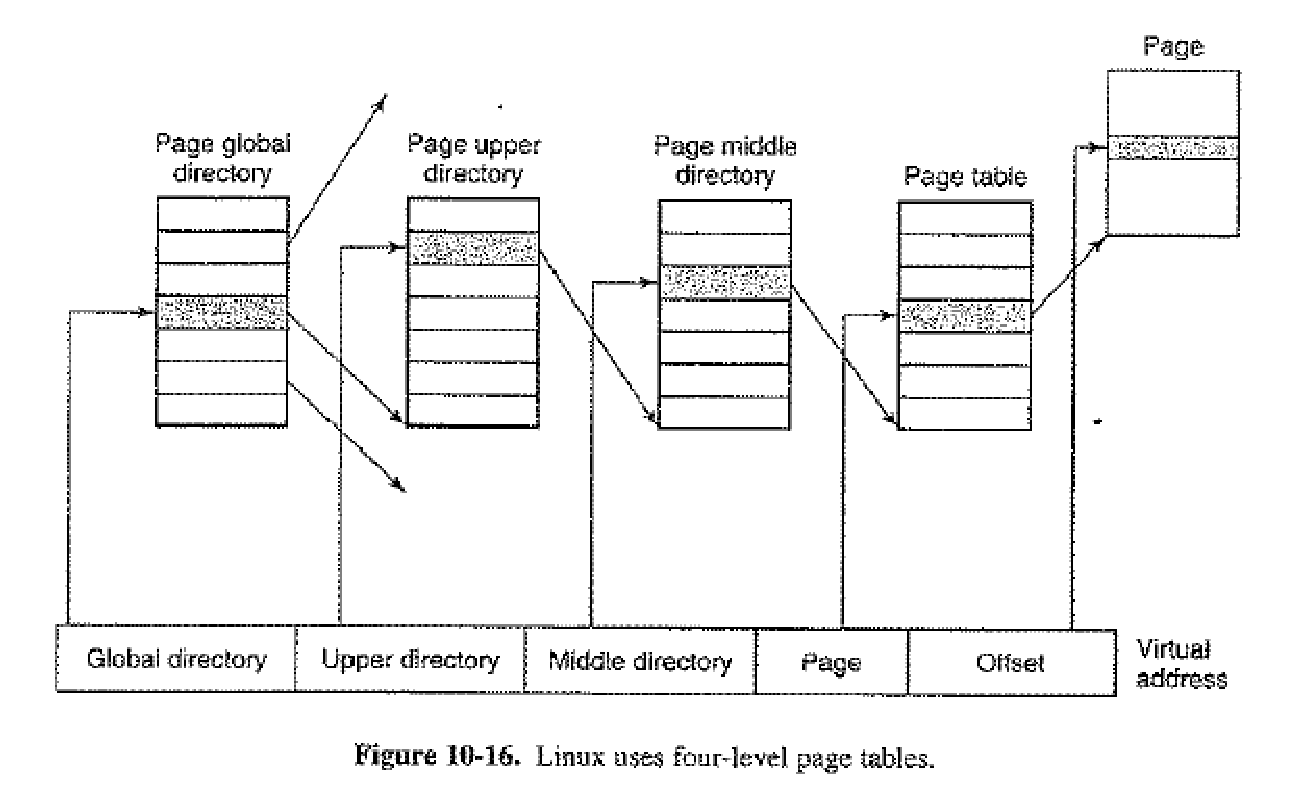
\includegraphics[width=6cm]{Seitentab.eps} 		
    
    
     \end{itemize}
    
\end{frame}


\begin{frame}
 
    \frametitle {Repräsentation des virtuellen Adressraumes}
    
    \framesubtitle {Paging in Linux}
    \begin{itemize}
         \item  Grundeinheit: Seite
         \item Grundidee / Definition Paging: \\
        \begin{quote}
         \textquotedblleft
         Paging ist ein Speicherverwaltungsverfahren, das auf der Strukturierung  des virtuellen Speichers 	in Seiten und der Strukturierung des realen Speichers in Seitenrahmen beruht.
    	\textquotedblright 	\end{quote}
 	 \item Nutzung 4-stufiger Seitentabellen in Linux
	 \item Realisierung sowohl durch kern als auch durch Page-Daemon
	 \item Demand - Paging - System unter Nutzung des Swap-Bereiches
	 \begin{itemize}
	 	\item Auslagerungspartition 
		\item Auslagerungsdateien
	\end{itemize}
    
    
     \end{itemize}
    
\end{frame}

\begin{frame}
	\frametitle{Repräsentation des virtuellen Adressraumes}\
	\framesubtitle {Der Seitenersetzungsalgorithmus}
 	\begin{itemize}
		\item per Page Frame Reclaiming Algorithmn
		\item Unterscheidung von vier Seitenarten:
	\end{itemize}	
		
		\begin{center}
		{\tiny
		\begin{tabular}{ l l }
 			 unreclaimable :&  reserviert/gesperrt/nicht auslagerbar \\
  			 swappable:       &  zurück auf Swap bzw Auslagerungspartition vor Neuanforderung\\
 			 syncable:		 &  zurück auf Platte, falls verändert\\
			 discardable:      & sofort anforderbar\\
		\end{tabular}
		}
		\end{center}
		
		zu beenden

			
    
\end{frame}



\section{Zusammenfassung}
\begin{frame}
    \frametitle{Zusammenfassung}
    \begin{itemize}
         \item   
    
    
    
     \end{itemize}
    
\end{frame}


\section{Literatur}
\begin{frame}
    \frametitle{Literatur}
    \begin{itemize}
         \item  Moderne Betriebssysteme \\
        		Andrew S. Tanenbaum - 2010
	\item	 UNIX - Wie funktioniert das Betriebssystem? \\
		Maurice J. Bach - 1991
	\item Betriebssysteme\\
		EIn Lehrbuch mit Übungen zur Systemprogrammierung in UNIX/ Linux \\
		E.Ehses, L. Köhler, P. Riemer, H. Stenzel, F. Victor - 2010	
    \end{itemize}
    
\end{frame}

\end{document}






